\documentclass{standalone}
\usepackage{tikz}
\usetikzlibrary{decorations.pathmorphing, arrows.meta}

\begin{document}
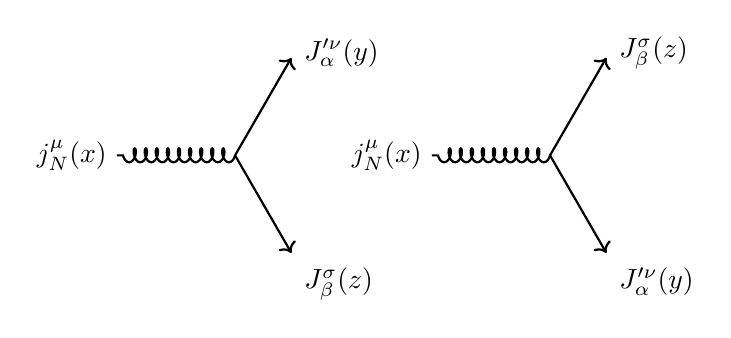
\begin{tikzpicture}[thick]
  % Left diagram
  \coordinate (a) at (0,0);
  \coordinate (b) at (60:1.5);
  \coordinate (c) at (300:1.5);
  \coordinate (d) at (180:1.5);

  \draw[decorate, decoration={coil, segment length=4pt}] (a) -- (d) node [left] {$j^{\mu}_N(x)$};
  \draw[->, shorten >=2pt] (a) -- (b) node [right] {$J^{\prime\nu}_{\alpha}(y)$};
  \draw[->, shorten >=2pt] (a) -- (c) node [below right] {$J^{\sigma}_{\beta}(z)$};

  % Right diagram
  \begin{scope}[shift={(4,0)}]
    \coordinate (a') at (0,0);
    \coordinate (b') at (60:1.5);
    \coordinate (c') at (300:1.5);
    \coordinate (d') at (180:1.5);

    \draw[decorate, decoration={coil, segment length=4pt}] (a') -- (d') node [left] {$j^{\mu}_N(x)$};
    \draw[->, shorten >=2pt] (a') -- (b') node [right] {$J^{\sigma}_{\beta}(z)$};
    \draw[->, shorten >=2pt] (a') -- (c') node [below right] {$J^{\prime\nu}_{\alpha}(y)$};
  \end{scope}
\end{tikzpicture}
\end{document}